% Created by tikzDevice version 0.12.6 on 2024-03-11 18:45:03
% !TEX encoding = UTF-8 Unicode
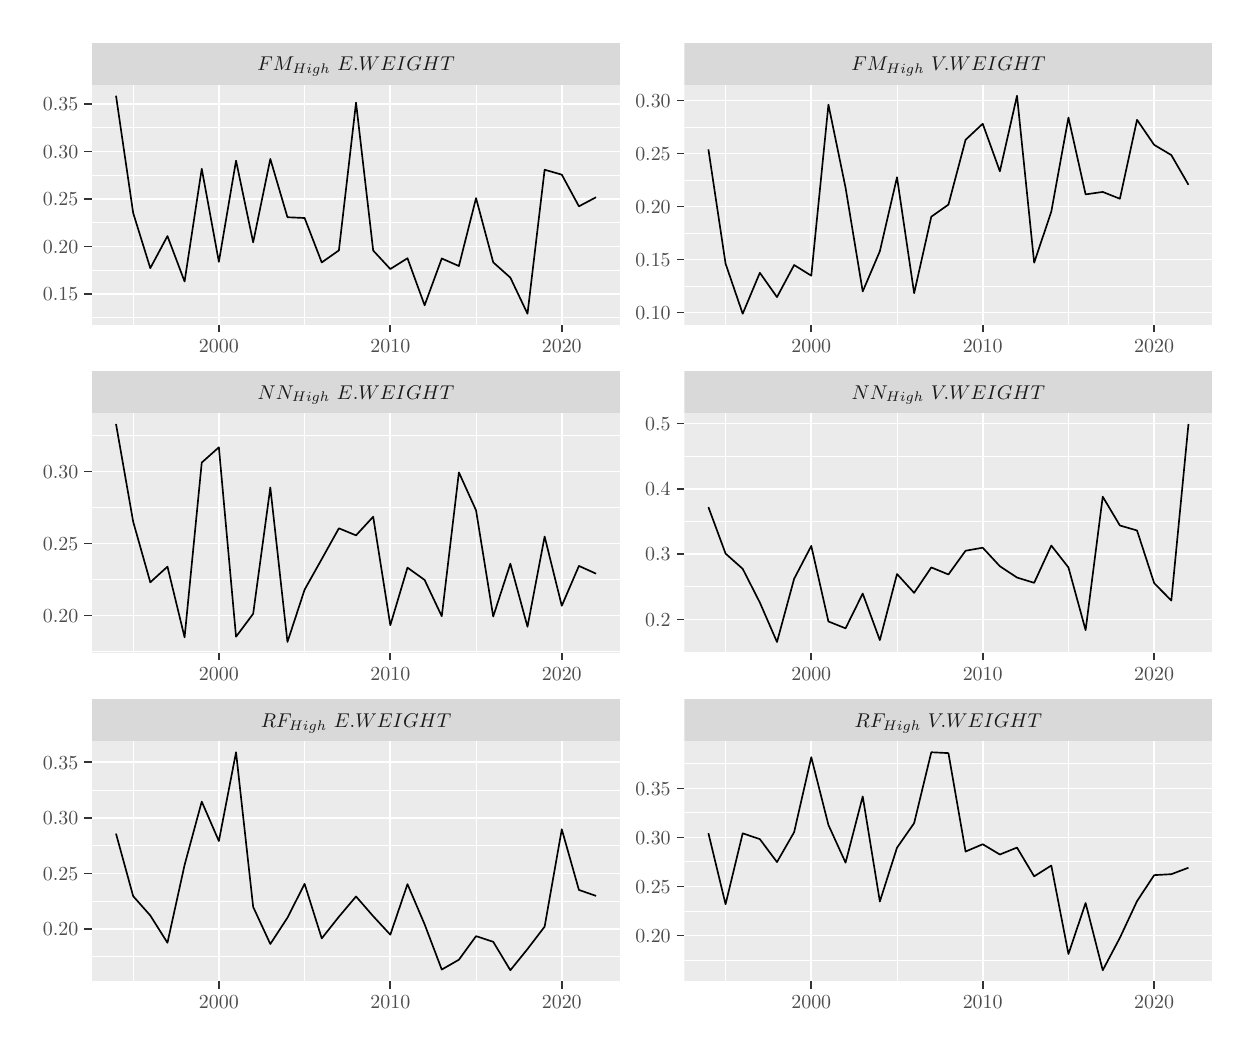
\begin{tikzpicture}[x=1pt,y=1pt]
\definecolor{fillColor}{RGB}{255,255,255}
\path[use as bounding box,fill=fillColor,fill opacity=0.00] (0,0) rectangle (433.62,361.35);
\begin{scope}
\path[clip] (  0.00,  0.00) rectangle (433.62,361.35);
\definecolor{drawColor}{RGB}{255,255,255}
\definecolor{fillColor}{RGB}{255,255,255}

\path[draw=drawColor,line width= 0.6pt,line join=round,line cap=round,fill=fillColor] (  0.00,  0.00) rectangle (433.62,361.35);
\end{scope}
\begin{scope}
\path[clip] ( 23.25,254.04) rectangle (214.06,340.69);
\definecolor{fillColor}{gray}{0.92}

\path[fill=fillColor] ( 23.25,254.04) rectangle (214.06,340.69);
\definecolor{drawColor}{RGB}{255,255,255}

\path[draw=drawColor,line width= 0.3pt,line join=round] ( 23.25,256.50) --
	(214.06,256.50);

\path[draw=drawColor,line width= 0.3pt,line join=round] ( 23.25,273.67) --
	(214.06,273.67);

\path[draw=drawColor,line width= 0.3pt,line join=round] ( 23.25,290.84) --
	(214.06,290.84);

\path[draw=drawColor,line width= 0.3pt,line join=round] ( 23.25,308.01) --
	(214.06,308.01);

\path[draw=drawColor,line width= 0.3pt,line join=round] ( 23.25,325.18) --
	(214.06,325.18);

\path[draw=drawColor,line width= 0.3pt,line join=round] ( 38.12,254.04) --
	( 38.12,340.69);

\path[draw=drawColor,line width= 0.3pt,line join=round] (100.07,254.04) --
	(100.07,340.69);

\path[draw=drawColor,line width= 0.3pt,line join=round] (162.02,254.04) --
	(162.02,340.69);

\path[draw=drawColor,line width= 0.6pt,line join=round] ( 23.25,265.09) --
	(214.06,265.09);

\path[draw=drawColor,line width= 0.6pt,line join=round] ( 23.25,282.26) --
	(214.06,282.26);

\path[draw=drawColor,line width= 0.6pt,line join=round] ( 23.25,299.43) --
	(214.06,299.43);

\path[draw=drawColor,line width= 0.6pt,line join=round] ( 23.25,316.60) --
	(214.06,316.60);

\path[draw=drawColor,line width= 0.6pt,line join=round] ( 23.25,333.77) --
	(214.06,333.77);

\path[draw=drawColor,line width= 0.6pt,line join=round] ( 69.09,254.04) --
	( 69.09,340.69);

\path[draw=drawColor,line width= 0.6pt,line join=round] (131.04,254.04) --
	(131.04,340.69);

\path[draw=drawColor,line width= 0.6pt,line join=round] (193.00,254.04) --
	(193.00,340.69);
\definecolor{drawColor}{RGB}{0,0,0}

\path[draw=drawColor,line width= 0.6pt,line join=round] ( 31.92,336.75) --
	( 38.12,294.39) --
	( 44.31,274.45) --
	( 50.51,286.04) --
	( 56.70,269.63) --
	( 62.90,310.37) --
	( 69.09,276.73) --
	( 75.29,313.29) --
	( 81.48,283.78) --
	( 87.68,313.91) --
	( 93.87,292.85) --
	(100.07,292.57) --
	(106.26,276.51) --
	(112.46,280.87) --
	(118.65,334.26) --
	(124.85,280.82) --
	(131.04,274.13) --
	(137.24,278.03) --
	(143.43,261.03) --
	(149.63,277.94) --
	(155.82,275.22) --
	(162.02,299.75) --
	(168.22,276.55) --
	(174.41,271.03) --
	(180.61,257.98) --
	(186.80,310.01) --
	(193.00,308.24) --
	(199.19,296.79) --
	(205.39,300.07);
\end{scope}
\begin{scope}
\path[clip] ( 23.25,135.43) rectangle (214.06,222.07);
\definecolor{fillColor}{gray}{0.92}

\path[fill=fillColor] ( 23.25,135.43) rectangle (214.06,222.07);
\definecolor{drawColor}{RGB}{255,255,255}

\path[draw=drawColor,line width= 0.3pt,line join=round] ( 23.25,135.94) --
	(214.06,135.94);

\path[draw=drawColor,line width= 0.3pt,line join=round] ( 23.25,161.96) --
	(214.06,161.96);

\path[draw=drawColor,line width= 0.3pt,line join=round] ( 23.25,187.98) --
	(214.06,187.98);

\path[draw=drawColor,line width= 0.3pt,line join=round] ( 23.25,214.00) --
	(214.06,214.00);

\path[draw=drawColor,line width= 0.3pt,line join=round] ( 38.12,135.43) --
	( 38.12,222.07);

\path[draw=drawColor,line width= 0.3pt,line join=round] (100.07,135.43) --
	(100.07,222.07);

\path[draw=drawColor,line width= 0.3pt,line join=round] (162.02,135.43) --
	(162.02,222.07);

\path[draw=drawColor,line width= 0.6pt,line join=round] ( 23.25,148.95) --
	(214.06,148.95);

\path[draw=drawColor,line width= 0.6pt,line join=round] ( 23.25,174.97) --
	(214.06,174.97);

\path[draw=drawColor,line width= 0.6pt,line join=round] ( 23.25,200.99) --
	(214.06,200.99);

\path[draw=drawColor,line width= 0.6pt,line join=round] ( 69.09,135.43) --
	( 69.09,222.07);

\path[draw=drawColor,line width= 0.6pt,line join=round] (131.04,135.43) --
	(131.04,222.07);

\path[draw=drawColor,line width= 0.6pt,line join=round] (193.00,135.43) --
	(193.00,222.07);
\definecolor{drawColor}{RGB}{0,0,0}

\path[draw=drawColor,line width= 0.6pt,line join=round] ( 31.92,218.14) --
	( 38.12,182.84) --
	( 44.31,160.94) --
	( 50.51,166.59) --
	( 56.70,141.06) --
	( 62.90,204.19) --
	( 69.09,209.72) --
	( 75.29,141.28) --
	( 81.48,149.55) --
	( 87.68,195.19) --
	( 93.87,139.36) --
	(100.07,158.28) --
	(106.26,169.32) --
	(112.46,180.45) --
	(118.65,177.89) --
	(124.85,184.63) --
	(131.04,145.43) --
	(137.24,166.23) --
	(143.43,161.79) --
	(149.63,148.67) --
	(155.82,200.65) --
	(162.02,186.92) --
	(168.22,148.57) --
	(174.41,167.65) --
	(180.61,144.88) --
	(186.80,177.47) --
	(193.00,152.44) --
	(199.19,166.85) --
	(205.39,164.05);
\end{scope}
\begin{scope}
\path[clip] ( 23.25, 16.81) rectangle (214.06,103.46);
\definecolor{fillColor}{gray}{0.92}

\path[fill=fillColor] ( 23.25, 16.81) rectangle (214.06,103.46);
\definecolor{drawColor}{RGB}{255,255,255}

\path[draw=drawColor,line width= 0.3pt,line join=round] ( 23.25, 25.58) --
	(214.06, 25.58);

\path[draw=drawColor,line width= 0.3pt,line join=round] ( 23.25, 45.68) --
	(214.06, 45.68);

\path[draw=drawColor,line width= 0.3pt,line join=round] ( 23.25, 65.79) --
	(214.06, 65.79);

\path[draw=drawColor,line width= 0.3pt,line join=round] ( 23.25, 85.89) --
	(214.06, 85.89);

\path[draw=drawColor,line width= 0.3pt,line join=round] ( 38.12, 16.81) --
	( 38.12,103.46);

\path[draw=drawColor,line width= 0.3pt,line join=round] (100.07, 16.81) --
	(100.07,103.46);

\path[draw=drawColor,line width= 0.3pt,line join=round] (162.02, 16.81) --
	(162.02,103.46);

\path[draw=drawColor,line width= 0.6pt,line join=round] ( 23.25, 35.63) --
	(214.06, 35.63);

\path[draw=drawColor,line width= 0.6pt,line join=round] ( 23.25, 55.74) --
	(214.06, 55.74);

\path[draw=drawColor,line width= 0.6pt,line join=round] ( 23.25, 75.84) --
	(214.06, 75.84);

\path[draw=drawColor,line width= 0.6pt,line join=round] ( 23.25, 95.95) --
	(214.06, 95.95);

\path[draw=drawColor,line width= 0.6pt,line join=round] ( 69.09, 16.81) --
	( 69.09,103.46);

\path[draw=drawColor,line width= 0.6pt,line join=round] (131.04, 16.81) --
	(131.04,103.46);

\path[draw=drawColor,line width= 0.6pt,line join=round] (193.00, 16.81) --
	(193.00,103.46);
\definecolor{drawColor}{RGB}{0,0,0}

\path[draw=drawColor,line width= 0.6pt,line join=round] ( 31.92, 70.11) --
	( 38.12, 47.52) --
	( 44.31, 40.53) --
	( 50.51, 30.68) --
	( 56.70, 58.79) --
	( 62.90, 81.69) --
	( 69.09, 67.43) --
	( 75.29, 99.52) --
	( 81.48, 43.63) --
	( 87.68, 30.23) --
	( 93.87, 39.73) --
	(100.07, 51.96) --
	(106.26, 32.26) --
	(112.46, 40.08) --
	(118.65, 47.41) --
	(124.85, 40.28) --
	(131.04, 33.60) --
	(137.24, 51.86) --
	(143.43, 37.36) --
	(149.63, 21.00) --
	(155.82, 24.55) --
	(162.02, 33.07) --
	(168.22, 31.04) --
	(174.41, 20.75) --
	(180.61, 28.41) --
	(186.80, 36.51) --
	(193.00, 71.68) --
	(199.19, 49.78) --
	(205.39, 47.61);
\end{scope}
\begin{scope}
\path[clip] (237.31,254.04) rectangle (428.12,340.69);
\definecolor{fillColor}{gray}{0.92}

\path[fill=fillColor] (237.31,254.04) rectangle (428.12,340.69);
\definecolor{drawColor}{RGB}{255,255,255}

\path[draw=drawColor,line width= 0.3pt,line join=round] (237.31,267.96) --
	(428.12,267.96);

\path[draw=drawColor,line width= 0.3pt,line join=round] (237.31,287.11) --
	(428.12,287.11);

\path[draw=drawColor,line width= 0.3pt,line join=round] (237.31,306.27) --
	(428.12,306.27);

\path[draw=drawColor,line width= 0.3pt,line join=round] (237.31,325.43) --
	(428.12,325.43);

\path[draw=drawColor,line width= 0.3pt,line join=round] (252.18,254.04) --
	(252.18,340.69);

\path[draw=drawColor,line width= 0.3pt,line join=round] (314.13,254.04) --
	(314.13,340.69);

\path[draw=drawColor,line width= 0.3pt,line join=round] (376.08,254.04) --
	(376.08,340.69);

\path[draw=drawColor,line width= 0.6pt,line join=round] (237.31,258.38) --
	(428.12,258.38);

\path[draw=drawColor,line width= 0.6pt,line join=round] (237.31,277.53) --
	(428.12,277.53);

\path[draw=drawColor,line width= 0.6pt,line join=round] (237.31,296.69) --
	(428.12,296.69);

\path[draw=drawColor,line width= 0.6pt,line join=round] (237.31,315.85) --
	(428.12,315.85);

\path[draw=drawColor,line width= 0.6pt,line join=round] (237.31,335.01) --
	(428.12,335.01);

\path[draw=drawColor,line width= 0.6pt,line join=round] (283.15,254.04) --
	(283.15,340.69);

\path[draw=drawColor,line width= 0.6pt,line join=round] (345.10,254.04) --
	(345.10,340.69);

\path[draw=drawColor,line width= 0.6pt,line join=round] (407.06,254.04) --
	(407.06,340.69);
\definecolor{drawColor}{RGB}{0,0,0}

\path[draw=drawColor,line width= 0.6pt,line join=round] (245.98,317.36) --
	(252.18,276.08) --
	(258.37,257.98) --
	(264.57,272.78) --
	(270.76,263.99) --
	(276.96,275.58) --
	(283.15,271.73) --
	(289.35,333.54) --
	(295.54,303.51) --
	(301.74,266.03) --
	(307.93,280.56) --
	(314.13,307.29) --
	(320.32,265.40) --
	(326.52,293.04) --
	(332.71,297.41) --
	(338.91,320.83) --
	(345.10,326.62) --
	(351.30,309.44) --
	(357.49,336.75) --
	(363.69,276.42) --
	(369.88,294.86) --
	(376.08,328.86) --
	(382.28,301.11) --
	(388.47,301.99) --
	(394.67,299.53) --
	(400.86,328.05) --
	(407.06,318.99) --
	(413.25,315.31) --
	(419.45,304.57);
\end{scope}
\begin{scope}
\path[clip] (237.31,135.43) rectangle (428.12,222.07);
\definecolor{fillColor}{gray}{0.92}

\path[fill=fillColor] (237.31,135.43) rectangle (428.12,222.07);
\definecolor{drawColor}{RGB}{255,255,255}

\path[draw=drawColor,line width= 0.3pt,line join=round] (237.31,135.76) --
	(428.12,135.76);

\path[draw=drawColor,line width= 0.3pt,line join=round] (237.31,159.34) --
	(428.12,159.34);

\path[draw=drawColor,line width= 0.3pt,line join=round] (237.31,182.91) --
	(428.12,182.91);

\path[draw=drawColor,line width= 0.3pt,line join=round] (237.31,206.49) --
	(428.12,206.49);

\path[draw=drawColor,line width= 0.3pt,line join=round] (252.18,135.43) --
	(252.18,222.07);

\path[draw=drawColor,line width= 0.3pt,line join=round] (314.13,135.43) --
	(314.13,222.07);

\path[draw=drawColor,line width= 0.3pt,line join=round] (376.08,135.43) --
	(376.08,222.07);

\path[draw=drawColor,line width= 0.6pt,line join=round] (237.31,147.55) --
	(428.12,147.55);

\path[draw=drawColor,line width= 0.6pt,line join=round] (237.31,171.12) --
	(428.12,171.12);

\path[draw=drawColor,line width= 0.6pt,line join=round] (237.31,194.70) --
	(428.12,194.70);

\path[draw=drawColor,line width= 0.6pt,line join=round] (237.31,218.28) --
	(428.12,218.28);

\path[draw=drawColor,line width= 0.6pt,line join=round] (283.15,135.43) --
	(283.15,222.07);

\path[draw=drawColor,line width= 0.6pt,line join=round] (345.10,135.43) --
	(345.10,222.07);

\path[draw=drawColor,line width= 0.6pt,line join=round] (407.06,135.43) --
	(407.06,222.07);
\definecolor{drawColor}{RGB}{0,0,0}

\path[draw=drawColor,line width= 0.6pt,line join=round] (245.98,188.10) --
	(252.18,171.31) --
	(258.37,165.80) --
	(264.57,153.62) --
	(270.76,139.36) --
	(276.96,162.21) --
	(283.15,174.08) --
	(289.35,146.78) --
	(295.54,144.30) --
	(301.74,156.87) --
	(307.93,140.03) --
	(314.13,163.93) --
	(320.32,157.12) --
	(326.52,166.31) --
	(332.71,163.76) --
	(338.91,172.34) --
	(345.10,173.43) --
	(351.30,166.74) --
	(357.49,162.65) --
	(363.69,160.74) --
	(369.88,174.21) --
	(376.08,166.30) --
	(382.28,143.64) --
	(388.47,191.87) --
	(394.67,181.46) --
	(400.86,179.66) --
	(407.06,160.62) --
	(413.25,154.33) --
	(419.45,218.14);
\end{scope}
\begin{scope}
\path[clip] (237.31, 16.81) rectangle (428.12,103.46);
\definecolor{fillColor}{gray}{0.92}

\path[fill=fillColor] (237.31, 16.81) rectangle (428.12,103.46);
\definecolor{drawColor}{RGB}{255,255,255}

\path[draw=drawColor,line width= 0.3pt,line join=round] (237.31, 24.46) --
	(428.12, 24.46);

\path[draw=drawColor,line width= 0.3pt,line join=round] (237.31, 42.18) --
	(428.12, 42.18);

\path[draw=drawColor,line width= 0.3pt,line join=round] (237.31, 59.90) --
	(428.12, 59.90);

\path[draw=drawColor,line width= 0.3pt,line join=round] (237.31, 77.62) --
	(428.12, 77.62);

\path[draw=drawColor,line width= 0.3pt,line join=round] (237.31, 95.34) --
	(428.12, 95.34);

\path[draw=drawColor,line width= 0.3pt,line join=round] (252.18, 16.81) --
	(252.18,103.46);

\path[draw=drawColor,line width= 0.3pt,line join=round] (314.13, 16.81) --
	(314.13,103.46);

\path[draw=drawColor,line width= 0.3pt,line join=round] (376.08, 16.81) --
	(376.08,103.46);

\path[draw=drawColor,line width= 0.6pt,line join=round] (237.31, 33.32) --
	(428.12, 33.32);

\path[draw=drawColor,line width= 0.6pt,line join=round] (237.31, 51.04) --
	(428.12, 51.04);

\path[draw=drawColor,line width= 0.6pt,line join=round] (237.31, 68.76) --
	(428.12, 68.76);

\path[draw=drawColor,line width= 0.6pt,line join=round] (237.31, 86.48) --
	(428.12, 86.48);

\path[draw=drawColor,line width= 0.6pt,line join=round] (283.15, 16.81) --
	(283.15,103.46);

\path[draw=drawColor,line width= 0.6pt,line join=round] (345.10, 16.81) --
	(345.10,103.46);

\path[draw=drawColor,line width= 0.6pt,line join=round] (407.06, 16.81) --
	(407.06,103.46);
\definecolor{drawColor}{RGB}{0,0,0}

\path[draw=drawColor,line width= 0.6pt,line join=round] (245.98, 70.27) --
	(252.18, 44.61) --
	(258.37, 70.23) --
	(264.57, 68.12) --
	(270.76, 59.84) --
	(276.96, 70.65) --
	(283.15, 97.74) --
	(289.35, 73.24) --
	(295.54, 59.62) --
	(301.74, 83.56) --
	(307.93, 45.60) --
	(314.13, 65.03) --
	(320.32, 73.91) --
	(326.52, 99.52) --
	(332.71, 99.21) --
	(338.91, 63.65) --
	(345.10, 66.28) --
	(351.30, 62.57) --
	(357.49, 65.08) --
	(363.69, 54.68) --
	(369.88, 58.59) --
	(376.08, 26.62) --
	(382.28, 45.05) --
	(388.47, 20.75) --
	(394.67, 32.48) --
	(400.86, 45.72) --
	(407.06, 55.12) --
	(413.25, 55.46) --
	(419.45, 57.80);
\end{scope}
\begin{scope}
\path[clip] ( 23.25,103.46) rectangle (214.06,118.62);
\definecolor{fillColor}{gray}{0.85}

\path[fill=fillColor] ( 23.25,103.46) rectangle (214.06,118.62);
\definecolor{drawColor}{gray}{0.10}

\node[text=drawColor,anchor=base,inner sep=0pt, outer sep=0pt, scale=  0.72] at (118.65,108.56) {$ RF _{ High } \ E.WEIGHT $};
\end{scope}
\begin{scope}
\path[clip] (237.31,103.46) rectangle (428.12,118.62);
\definecolor{fillColor}{gray}{0.85}

\path[fill=fillColor] (237.31,103.46) rectangle (428.12,118.62);
\definecolor{drawColor}{gray}{0.10}

\node[text=drawColor,anchor=base,inner sep=0pt, outer sep=0pt, scale=  0.72] at (332.71,108.56) {$ RF _{ High } \ V.WEIGHT $};
\end{scope}
\begin{scope}
\path[clip] ( 23.25,222.07) rectangle (214.06,237.23);
\definecolor{fillColor}{gray}{0.85}

\path[fill=fillColor] ( 23.25,222.07) rectangle (214.06,237.23);
\definecolor{drawColor}{gray}{0.10}

\node[text=drawColor,anchor=base,inner sep=0pt, outer sep=0pt, scale=  0.72] at (118.65,227.17) {$ NN _{ High } \ E.WEIGHT $};
\end{scope}
\begin{scope}
\path[clip] (237.31,222.07) rectangle (428.12,237.23);
\definecolor{fillColor}{gray}{0.85}

\path[fill=fillColor] (237.31,222.07) rectangle (428.12,237.23);
\definecolor{drawColor}{gray}{0.10}

\node[text=drawColor,anchor=base,inner sep=0pt, outer sep=0pt, scale=  0.72] at (332.71,227.17) {$ NN _{ High } \ V.WEIGHT $};
\end{scope}
\begin{scope}
\path[clip] ( 23.25,340.69) rectangle (214.06,355.85);
\definecolor{fillColor}{gray}{0.85}

\path[fill=fillColor] ( 23.25,340.69) rectangle (214.06,355.85);
\definecolor{drawColor}{gray}{0.10}

\node[text=drawColor,anchor=base,inner sep=0pt, outer sep=0pt, scale=  0.72] at (118.65,345.79) {$ FM _{ High } \ E.WEIGHT $};
\end{scope}
\begin{scope}
\path[clip] (237.31,340.69) rectangle (428.12,355.85);
\definecolor{fillColor}{gray}{0.85}

\path[fill=fillColor] (237.31,340.69) rectangle (428.12,355.85);
\definecolor{drawColor}{gray}{0.10}

\node[text=drawColor,anchor=base,inner sep=0pt, outer sep=0pt, scale=  0.72] at (332.71,345.79) {$ FM _{ High } \ V.WEIGHT $};
\end{scope}
\begin{scope}
\path[clip] (  0.00,  0.00) rectangle (433.62,361.35);
\definecolor{drawColor}{gray}{0.20}

\path[draw=drawColor,line width= 0.6pt,line join=round] ( 69.09, 14.06) --
	( 69.09, 16.81);

\path[draw=drawColor,line width= 0.6pt,line join=round] (131.04, 14.06) --
	(131.04, 16.81);

\path[draw=drawColor,line width= 0.6pt,line join=round] (193.00, 14.06) --
	(193.00, 16.81);
\end{scope}
\begin{scope}
\path[clip] (  0.00,  0.00) rectangle (433.62,361.35);
\definecolor{drawColor}{gray}{0.30}

\node[text=drawColor,anchor=base,inner sep=0pt, outer sep=0pt, scale=  0.72] at ( 69.09,  6.90) {2000};

\node[text=drawColor,anchor=base,inner sep=0pt, outer sep=0pt, scale=  0.72] at (131.04,  6.90) {2010};

\node[text=drawColor,anchor=base,inner sep=0pt, outer sep=0pt, scale=  0.72] at (193.00,  6.90) {2020};
\end{scope}
\begin{scope}
\path[clip] (  0.00,  0.00) rectangle (433.62,361.35);
\definecolor{drawColor}{gray}{0.20}

\path[draw=drawColor,line width= 0.6pt,line join=round] (283.15, 14.06) --
	(283.15, 16.81);

\path[draw=drawColor,line width= 0.6pt,line join=round] (345.10, 14.06) --
	(345.10, 16.81);

\path[draw=drawColor,line width= 0.6pt,line join=round] (407.06, 14.06) --
	(407.06, 16.81);
\end{scope}
\begin{scope}
\path[clip] (  0.00,  0.00) rectangle (433.62,361.35);
\definecolor{drawColor}{gray}{0.30}

\node[text=drawColor,anchor=base,inner sep=0pt, outer sep=0pt, scale=  0.72] at (283.15,  6.90) {2000};

\node[text=drawColor,anchor=base,inner sep=0pt, outer sep=0pt, scale=  0.72] at (345.10,  6.90) {2010};

\node[text=drawColor,anchor=base,inner sep=0pt, outer sep=0pt, scale=  0.72] at (407.06,  6.90) {2020};
\end{scope}
\begin{scope}
\path[clip] (  0.00,  0.00) rectangle (433.62,361.35);
\definecolor{drawColor}{gray}{0.20}

\path[draw=drawColor,line width= 0.6pt,line join=round] ( 69.09,132.68) --
	( 69.09,135.43);

\path[draw=drawColor,line width= 0.6pt,line join=round] (131.04,132.68) --
	(131.04,135.43);

\path[draw=drawColor,line width= 0.6pt,line join=round] (193.00,132.68) --
	(193.00,135.43);
\end{scope}
\begin{scope}
\path[clip] (  0.00,  0.00) rectangle (433.62,361.35);
\definecolor{drawColor}{gray}{0.30}

\node[text=drawColor,anchor=base,inner sep=0pt, outer sep=0pt, scale=  0.72] at ( 69.09,125.52) {2000};

\node[text=drawColor,anchor=base,inner sep=0pt, outer sep=0pt, scale=  0.72] at (131.04,125.52) {2010};

\node[text=drawColor,anchor=base,inner sep=0pt, outer sep=0pt, scale=  0.72] at (193.00,125.52) {2020};
\end{scope}
\begin{scope}
\path[clip] (  0.00,  0.00) rectangle (433.62,361.35);
\definecolor{drawColor}{gray}{0.20}

\path[draw=drawColor,line width= 0.6pt,line join=round] (283.15,132.68) --
	(283.15,135.43);

\path[draw=drawColor,line width= 0.6pt,line join=round] (345.10,132.68) --
	(345.10,135.43);

\path[draw=drawColor,line width= 0.6pt,line join=round] (407.06,132.68) --
	(407.06,135.43);
\end{scope}
\begin{scope}
\path[clip] (  0.00,  0.00) rectangle (433.62,361.35);
\definecolor{drawColor}{gray}{0.30}

\node[text=drawColor,anchor=base,inner sep=0pt, outer sep=0pt, scale=  0.72] at (283.15,125.52) {2000};

\node[text=drawColor,anchor=base,inner sep=0pt, outer sep=0pt, scale=  0.72] at (345.10,125.52) {2010};

\node[text=drawColor,anchor=base,inner sep=0pt, outer sep=0pt, scale=  0.72] at (407.06,125.52) {2020};
\end{scope}
\begin{scope}
\path[clip] (  0.00,  0.00) rectangle (433.62,361.35);
\definecolor{drawColor}{gray}{0.20}

\path[draw=drawColor,line width= 0.6pt,line join=round] ( 69.09,251.29) --
	( 69.09,254.04);

\path[draw=drawColor,line width= 0.6pt,line join=round] (131.04,251.29) --
	(131.04,254.04);

\path[draw=drawColor,line width= 0.6pt,line join=round] (193.00,251.29) --
	(193.00,254.04);
\end{scope}
\begin{scope}
\path[clip] (  0.00,  0.00) rectangle (433.62,361.35);
\definecolor{drawColor}{gray}{0.30}

\node[text=drawColor,anchor=base,inner sep=0pt, outer sep=0pt, scale=  0.72] at ( 69.09,244.13) {2000};

\node[text=drawColor,anchor=base,inner sep=0pt, outer sep=0pt, scale=  0.72] at (131.04,244.13) {2010};

\node[text=drawColor,anchor=base,inner sep=0pt, outer sep=0pt, scale=  0.72] at (193.00,244.13) {2020};
\end{scope}
\begin{scope}
\path[clip] (  0.00,  0.00) rectangle (433.62,361.35);
\definecolor{drawColor}{gray}{0.20}

\path[draw=drawColor,line width= 0.6pt,line join=round] (283.15,251.29) --
	(283.15,254.04);

\path[draw=drawColor,line width= 0.6pt,line join=round] (345.10,251.29) --
	(345.10,254.04);

\path[draw=drawColor,line width= 0.6pt,line join=round] (407.06,251.29) --
	(407.06,254.04);
\end{scope}
\begin{scope}
\path[clip] (  0.00,  0.00) rectangle (433.62,361.35);
\definecolor{drawColor}{gray}{0.30}

\node[text=drawColor,anchor=base,inner sep=0pt, outer sep=0pt, scale=  0.72] at (283.15,244.13) {2000};

\node[text=drawColor,anchor=base,inner sep=0pt, outer sep=0pt, scale=  0.72] at (345.10,244.13) {2010};

\node[text=drawColor,anchor=base,inner sep=0pt, outer sep=0pt, scale=  0.72] at (407.06,244.13) {2020};
\end{scope}
\begin{scope}
\path[clip] (  0.00,  0.00) rectangle (433.62,361.35);
\definecolor{drawColor}{gray}{0.30}

\node[text=drawColor,anchor=base east,inner sep=0pt, outer sep=0pt, scale=  0.72] at (232.36,255.90) {0.10};

\node[text=drawColor,anchor=base east,inner sep=0pt, outer sep=0pt, scale=  0.72] at (232.36,275.05) {0.15};

\node[text=drawColor,anchor=base east,inner sep=0pt, outer sep=0pt, scale=  0.72] at (232.36,294.21) {0.20};

\node[text=drawColor,anchor=base east,inner sep=0pt, outer sep=0pt, scale=  0.72] at (232.36,313.37) {0.25};

\node[text=drawColor,anchor=base east,inner sep=0pt, outer sep=0pt, scale=  0.72] at (232.36,332.53) {0.30};
\end{scope}
\begin{scope}
\path[clip] (  0.00,  0.00) rectangle (433.62,361.35);
\definecolor{drawColor}{gray}{0.20}

\path[draw=drawColor,line width= 0.6pt,line join=round] (234.56,258.38) --
	(237.31,258.38);

\path[draw=drawColor,line width= 0.6pt,line join=round] (234.56,277.53) --
	(237.31,277.53);

\path[draw=drawColor,line width= 0.6pt,line join=round] (234.56,296.69) --
	(237.31,296.69);

\path[draw=drawColor,line width= 0.6pt,line join=round] (234.56,315.85) --
	(237.31,315.85);

\path[draw=drawColor,line width= 0.6pt,line join=round] (234.56,335.01) --
	(237.31,335.01);
\end{scope}
\begin{scope}
\path[clip] (  0.00,  0.00) rectangle (433.62,361.35);
\definecolor{drawColor}{gray}{0.30}

\node[text=drawColor,anchor=base east,inner sep=0pt, outer sep=0pt, scale=  0.72] at (232.36,145.07) {0.2};

\node[text=drawColor,anchor=base east,inner sep=0pt, outer sep=0pt, scale=  0.72] at (232.36,168.65) {0.3};

\node[text=drawColor,anchor=base east,inner sep=0pt, outer sep=0pt, scale=  0.72] at (232.36,192.22) {0.4};

\node[text=drawColor,anchor=base east,inner sep=0pt, outer sep=0pt, scale=  0.72] at (232.36,215.80) {0.5};
\end{scope}
\begin{scope}
\path[clip] (  0.00,  0.00) rectangle (433.62,361.35);
\definecolor{drawColor}{gray}{0.20}

\path[draw=drawColor,line width= 0.6pt,line join=round] (234.56,147.55) --
	(237.31,147.55);

\path[draw=drawColor,line width= 0.6pt,line join=round] (234.56,171.12) --
	(237.31,171.12);

\path[draw=drawColor,line width= 0.6pt,line join=round] (234.56,194.70) --
	(237.31,194.70);

\path[draw=drawColor,line width= 0.6pt,line join=round] (234.56,218.28) --
	(237.31,218.28);
\end{scope}
\begin{scope}
\path[clip] (  0.00,  0.00) rectangle (433.62,361.35);
\definecolor{drawColor}{gray}{0.30}

\node[text=drawColor,anchor=base east,inner sep=0pt, outer sep=0pt, scale=  0.72] at (232.36, 30.84) {0.20};

\node[text=drawColor,anchor=base east,inner sep=0pt, outer sep=0pt, scale=  0.72] at (232.36, 48.56) {0.25};

\node[text=drawColor,anchor=base east,inner sep=0pt, outer sep=0pt, scale=  0.72] at (232.36, 66.28) {0.30};

\node[text=drawColor,anchor=base east,inner sep=0pt, outer sep=0pt, scale=  0.72] at (232.36, 84.00) {0.35};
\end{scope}
\begin{scope}
\path[clip] (  0.00,  0.00) rectangle (433.62,361.35);
\definecolor{drawColor}{gray}{0.20}

\path[draw=drawColor,line width= 0.6pt,line join=round] (234.56, 33.32) --
	(237.31, 33.32);

\path[draw=drawColor,line width= 0.6pt,line join=round] (234.56, 51.04) --
	(237.31, 51.04);

\path[draw=drawColor,line width= 0.6pt,line join=round] (234.56, 68.76) --
	(237.31, 68.76);

\path[draw=drawColor,line width= 0.6pt,line join=round] (234.56, 86.48) --
	(237.31, 86.48);
\end{scope}
\begin{scope}
\path[clip] (  0.00,  0.00) rectangle (433.62,361.35);
\definecolor{drawColor}{gray}{0.30}

\node[text=drawColor,anchor=base east,inner sep=0pt, outer sep=0pt, scale=  0.72] at ( 18.30,262.61) {0.15};

\node[text=drawColor,anchor=base east,inner sep=0pt, outer sep=0pt, scale=  0.72] at ( 18.30,279.78) {0.20};

\node[text=drawColor,anchor=base east,inner sep=0pt, outer sep=0pt, scale=  0.72] at ( 18.30,296.95) {0.25};

\node[text=drawColor,anchor=base east,inner sep=0pt, outer sep=0pt, scale=  0.72] at ( 18.30,314.12) {0.30};

\node[text=drawColor,anchor=base east,inner sep=0pt, outer sep=0pt, scale=  0.72] at ( 18.30,331.29) {0.35};
\end{scope}
\begin{scope}
\path[clip] (  0.00,  0.00) rectangle (433.62,361.35);
\definecolor{drawColor}{gray}{0.20}

\path[draw=drawColor,line width= 0.6pt,line join=round] ( 20.50,265.09) --
	( 23.25,265.09);

\path[draw=drawColor,line width= 0.6pt,line join=round] ( 20.50,282.26) --
	( 23.25,282.26);

\path[draw=drawColor,line width= 0.6pt,line join=round] ( 20.50,299.43) --
	( 23.25,299.43);

\path[draw=drawColor,line width= 0.6pt,line join=round] ( 20.50,316.60) --
	( 23.25,316.60);

\path[draw=drawColor,line width= 0.6pt,line join=round] ( 20.50,333.77) --
	( 23.25,333.77);
\end{scope}
\begin{scope}
\path[clip] (  0.00,  0.00) rectangle (433.62,361.35);
\definecolor{drawColor}{gray}{0.30}

\node[text=drawColor,anchor=base east,inner sep=0pt, outer sep=0pt, scale=  0.72] at ( 18.30,146.47) {0.20};

\node[text=drawColor,anchor=base east,inner sep=0pt, outer sep=0pt, scale=  0.72] at ( 18.30,172.49) {0.25};

\node[text=drawColor,anchor=base east,inner sep=0pt, outer sep=0pt, scale=  0.72] at ( 18.30,198.51) {0.30};
\end{scope}
\begin{scope}
\path[clip] (  0.00,  0.00) rectangle (433.62,361.35);
\definecolor{drawColor}{gray}{0.20}

\path[draw=drawColor,line width= 0.6pt,line join=round] ( 20.50,148.95) --
	( 23.25,148.95);

\path[draw=drawColor,line width= 0.6pt,line join=round] ( 20.50,174.97) --
	( 23.25,174.97);

\path[draw=drawColor,line width= 0.6pt,line join=round] ( 20.50,200.99) --
	( 23.25,200.99);
\end{scope}
\begin{scope}
\path[clip] (  0.00,  0.00) rectangle (433.62,361.35);
\definecolor{drawColor}{gray}{0.30}

\node[text=drawColor,anchor=base east,inner sep=0pt, outer sep=0pt, scale=  0.72] at ( 18.30, 33.15) {0.20};

\node[text=drawColor,anchor=base east,inner sep=0pt, outer sep=0pt, scale=  0.72] at ( 18.30, 53.26) {0.25};

\node[text=drawColor,anchor=base east,inner sep=0pt, outer sep=0pt, scale=  0.72] at ( 18.30, 73.36) {0.30};

\node[text=drawColor,anchor=base east,inner sep=0pt, outer sep=0pt, scale=  0.72] at ( 18.30, 93.47) {0.35};
\end{scope}
\begin{scope}
\path[clip] (  0.00,  0.00) rectangle (433.62,361.35);
\definecolor{drawColor}{gray}{0.20}

\path[draw=drawColor,line width= 0.6pt,line join=round] ( 20.50, 35.63) --
	( 23.25, 35.63);

\path[draw=drawColor,line width= 0.6pt,line join=round] ( 20.50, 55.74) --
	( 23.25, 55.74);

\path[draw=drawColor,line width= 0.6pt,line join=round] ( 20.50, 75.84) --
	( 23.25, 75.84);

\path[draw=drawColor,line width= 0.6pt,line join=round] ( 20.50, 95.95) --
	( 23.25, 95.95);
\end{scope}
\end{tikzpicture}
